\section{System Design}
In this section we describe key aspects of our system design which increase the throughput of inter node communication. First of all it is worth to note that even with one TCP connection, it is possible to saturate the network link usage, if the sending and receiving processes send and receive byte arrays without any delay even with 256 bytes array messages. However serializing java object messages to byte arrays and deserializing byte arrays back to java objects take considerable amount of time. Hence the key aspect of  improving the system performance is to reduce this message processing delay. We use multitasking and bulk message serializing to solve this problem. 

In this design, we use thread pools both at client side and server side to processes messages while sharing a single TCP connection. Firstly both thread pools access underline connection resource only to send receive byte arrays making message serialization and deserialization process parallel. Secondly it serializes messages together to improve performance of the serialization process.  Figure \ref{interprocess} shows the design involved in sending a message from one process to another. 

Lets assume client side process requires to send a set of messages to server side process. In order to send these messages first the client process threads send these messages to its \textit{ElementContainer}. \textit{ElementContainer} holds all the streams (this is an abstraction of a link in the process graph) to which these messages need to be send and it pushes each message to all the streams. Stream decides the target node and buffers messages for a configured amount of size. Then it passes the buffered  message list along the target node details to \textit{ConnectionManager} which holds \textit{ClientConnection}s for each node. \textit{ConnectionManager} serializes the message list and sends the byte array to correct \textit{ClientConnection} using the target node. \textit{ClientConnection} uses the \textit{DataOutput} which wraps the TCP connection to send message to server side. 

At the server side there is a set of \textit{ServerTask}s which reads receiving messages from a pool of \textit{DataInput} streams available in the \textit{ServerConnection} (we register these connections at the connections creating time) and send them to receiving processes. First a server task acquires a \textit{DataInput} stream and reads the binary message and release it. Then it deserializes the binary message using the sending process id to identify the event type.  After that it passes this message to the \textit{WorkerContainer} which holds all processes. Finally \textit{WorkerContainer} dispatches this message to correct process using receiving process id. Message ordering happens at the process level if required. 

\begin{figure}[!tii]
        \centering
        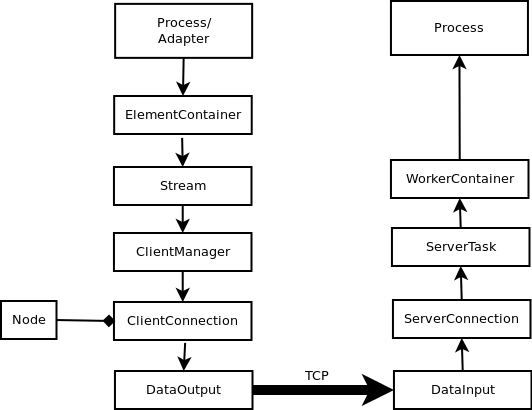
\includegraphics[width=3.0in]{interprocess.png}
        \caption{Communication between two Process}
        \label{interprocess}
\end{figure}
